\documentclass{article}
\usepackage{amsmath}
\usepackage{amssymb}
\usepackage{graphicx}
\usepackage{tikz}
\usepackage{pgfplots}
\pgfplotsset{compat=1.15}
\usepackage{mathrsfs}
\usetikzlibrary{arrows}

\begin{document}
%colori tex
\definecolor{wewdxt}{rgb}{0.43137254901960786,0.42745098039215684,0.45098039215686275}
\title{Analisi II - Integrali}
\author{Marco Delton\thanks{esercizi della prof.ssa \textit{Chiara Bianchini}}}
\date{A.A. 2025/26}

\maketitle

\begin{enumerate}
    %ES. 1
\item Scrivere i seguenti domini come unione di domini normali:
    \begin{enumerate}
        %P. 1
        \item \begin{tikzpicture}[scale=0.5]
            %assi
            \draw[->] (-1,0) -- (3,0) node[right] {$x$};
            \draw[->] (0,-1) -- (0,3) node[above] {$y$};
            %grafico
            \draw (0,1) -- (1,1);
            \draw[dashed] (1,1) -- (1,0);
            \draw (1,1) -- (2,0);
            \draw (1,1) node[above right] {\tiny{(1,1)}};
        \end{tikzpicture}
        
        %P. 2
        \item \begin{tikzpicture}
            %assi
            \draw[->] (-1,0) -- (4,0) node[right] {$x$};
            \draw[dashed] (2,1) -- (2,0);
            \draw[->] (0,-1) -- (0,2) node[above] {$y$};
            %grafico
            \draw (0,0) -- (2,1);
            \draw (2,1) -- (3,0);
            \draw (2,1) node[above right] {\tiny{(2,1)}};
        \end{tikzpicture}

        %P. 3
        \item 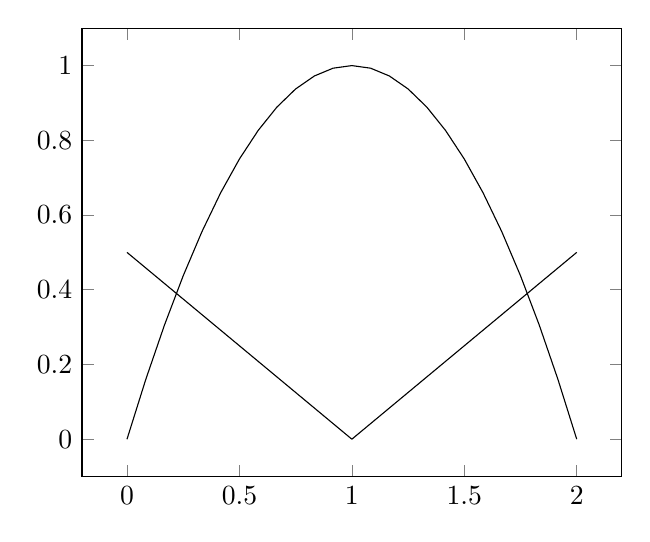
\begin{tikzpicture}
            \begin{axis}
                \addplot[domain=0:1] {-(x/2)+1/2};
                \addplot[domain=1:2] {(x/2)-1/2};
                \addplot[domain=0:2] {-x^2 + 2*x};
            \end{axis}
        \end{tikzpicture}

        %P. 4
        \item \begin{tikzpicture}
            \begin{axis}
                \addplot[domain=-1:1,samples=200] {x^2-1};
                \addplot[domain=-1:1,samples=500] {sqrt(1-x^2)};
            \end{axis}
        \end{tikzpicture}
    \end{enumerate}$\\$

    %ES. 2
    \item Disegnare i seguenti domini:\begin{enumerate}
        \item $E_1=\left\{(x,y)\in\mathbb{R}^2:\begin{matrix}
        0\leq x\leq1\\
        0\leq y\leq 1-2x
        \end{matrix}\right\}$

        \item $E_2=\left\{(x,y)\in\mathbb{R}^2:\begin{matrix}
        -1\leq x\leq1\\
        0\leq y\leq 2-\sqrt{1-x^2}
        \end{matrix}\right\}$

        \item $E_3=\left\{(x,y)\in\mathbb{R}^2:\begin{matrix}
        x^2+y^2+2x\geq 0\\
        x^2+y^2-2x\geq 0\\
        x^2+y^2 \leq 4
        \end{matrix}\right\}$

        \item $E_4=\left\{(x,y)\in\mathbb{R}^2:\begin{matrix}
        \left|x+y-\frac{1}{2}\right|\leq \frac{1}{2}\\
        xy \geq 1
        \end{matrix}\right\}$

        \item $E_5=\left\{(x,y)\in\mathbb{R}^2:\begin{matrix}
        (x-1)^2+y^2\leq 4\\
        (x+1)^2+y^2\leq 4\\
        y \leq 0
        \end{matrix}\right\}$

        \item $E_6=\left\{(x,y)\in\mathbb{R}^2:\begin{matrix}
        x\in [0,\pi]\\
        y\in[0,\sin x]
        \end{matrix}\right\}\\$
    \end{enumerate}

    %ES. 3
    \item Calcolare:
    \[\iint_D(x^2+y^2) \ dx \ dy \quad \text{su } D=\left\{\begin{matrix}
    0 \leq x \leq 1\\
    0 \leq y \leq 1-x
    \end{matrix}\right\}\\\]

    %ES. 4
    \item Calcolare:
    \[\iint_Ex^2 \ dx \ dy \quad \text{su } E=\left\{\begin{matrix}
    x^2+y^2 \leq 1\\
    y \geq x^2-1
    \end{matrix}\right\}\\\]

    %ES. 5
    \item Calcolare:
    \[\iint_D2ye^x \ dx \ dy \quad \text{su } D=E_3\quad(\text{dell'es. 2})\\\]

    %ES. 6
    \item Calcolare:
    \[\iint_D\frac{1}{1+y} \ dx \ dy\quad \text{su } D=E_2\quad(\text{dell' es. 2})\\\]

    %ES. 7
    \item Calcolare il baricentro di $E_6$ (dell' es. 2)$\\$
    
    %ES. 8
    \item Determinare il momento di inerzia di $E_6$ (dell' es. 2) rispetto agli assi $x$ e $y$$\\$

    %ES. 9
    \item Determinare il volume del toro generico$\\$
    
    %ES. 10
    \item Calcolare il baricentro di una lamina piana a forma di semicerchio$\\$

    %ES. 11
    \item Calcolare l'area e il baricentro di $E_4$ (dell' es. 2)$\\$
    
    %ES. 12
    \item Calcolare il baricentro di $E_5$ (dell' es. 2)$\\$
    
    %ES. 13
    \item Calcolare l'area della porzione di spirale di Archimede (scritta in coordinate polari):
    \[E=\left\{(\theta,\rho):\theta\in \left[\frac{\pi}{4},\frac{9\pi}{4}\right],\quad\rho\in [\theta,\theta +2\pi]\right\}\\\]

    %ES. 14
    \item Calcolare:
    \[\iint_Dx\arctan{\left(\frac{x}{y}\right)} \ dx \ dy\quad\text{su } D=\left\{\begin{matrix}
    x^2+y^2 \leq 4\\
    x^2+y^2 \leq 1\\
    x \geq 0\\
    y \geq 0
    \end{matrix}\right\}\\\]

    %ES. 15
    \item Calcolare:
    \[\iint_T\frac{x^2y}{x^2+y^2} \ dx \ dy\quad\text{su } T=\left\{\begin{matrix}
    y \geq 0\\
    a^2 \leq x^2+y^2 \leq b^2
    \end{matrix}\right\}\\\]

    %ES. 16
    \item Calcolare l'area della regione di piano: 
    \[\left\{\begin{matrix}
    4\leq 4x^2+y^2 \leq 16\\
    \frac{x}{2} \leq y \leq 2x
    \end{matrix}\right\}\\\]

    %ES. 17
    \item Calcolare il volume di E:
    \[E=\left\{\begin{matrix}
    x > 0\\
    y > 0\\
    \sqrt{x}+\sqrt{y} \leq 1\\
    0 \leq z \leq \sqrt{xy}
    \end{matrix}\right\}\]

    %ES. 18
    \item Calcolare: 
    \[\iint_E(2x^2-2x-xy+y)\cdot\left(\cos{(y-x^2)(y-2x)}\right)\cdot\ln{\left|\cos{(y-2x)}\right|} \ dx \ dy\\\]

    %ES. 19
    \item Calcolare:
    \[\iiint_D\sqrt{x^2+y^2} \ dx \ dy \ dz\]
    Dove $D$ è delimitato dalla falda superiore del cono $z^2=x^2+y^2$ e dal piano $z=1\\$

    %ES. 20
    \item Calcolare la massa del solido compreso tra due superfici sferiche concentriche di raggi $a$ e $b$ con $0<a<b$, la cui densità è il quadrato della distanza del punto dal centro $\\$
    
    %ES. 21
    \item Calcolare:
    \[\iint_Ex\frac{2-3y^2}{\left(2-y^2\right)^2} \ dx \ dy\quad\text{su } E=\left\{\begin{matrix}
    0\leq x \leq 2\\
    0\leq y \leq \left(1-x\right)^2
    \end{matrix}\right\}\\\]

    %ES. 22
    \item Calcolare: 
    \[\iint_E\frac{y}{\sqrt{2+x+y^2}} \ dx \ dy\quad\text{su } E=\left\{\begin{matrix}
    x^2+y^2\leq1\\
    x+y+\frac{1}{2}\leq0
    \end{matrix}\right\}\\\]

    %ES. 23
    \item Calcolare: 
    \[\iint_E\frac{x+2y}{2y^2+\sqrt{3}xy} \ dx \ dy\quad\text{su } E=\left\{\begin{matrix}
    1\leq\frac{x^2}{3}+y^2\leq4\\
    |x|\leq|y|
    \end{matrix}\right\}\\\]

    %ES. 24
    \item Sia $E=\left\{(x,y,z)\in\mathbb{R}^3:\begin{matrix}
    y=0\\
    (x-2)^2+z^2\leq1\\
    z\geq\frac{1}{\sqrt{2}}
    \end{matrix}\right\}\\$
    Sia $T$ ottenuto ruotando $E$ attorno all'asse $z$.\\
    Calcolare: 
    \[\iiint_T\frac{1}{\sqrt{x^2+y^2}(1+z^2)} \ dx \ dy \ dz\\\]

    %ES.25
    \item Calcolare:
    \[\iiint_Cx^2 \ dx \ dy \ dz\]
    dove $C$ è la parte, compresa tra i piani $z=0$ e $z=1$, del cono che proietta l'ellisse $x^2+\left(\frac{y}{2}\right)^2\leq1,\quad z=1$, dall'origine delle coordinate $\\$

    %ES. 26
    \item Calcolare: 
    \[\iiint_Ez \ dx \ dy \ dz\]
    dove $E$ è il solido contenuto nel semipiano $\{x>0\}$, delimitato dai piani $x=0$,$z=0$, dalla sfera $x^2+y^2+z^2=\frac{1}{4}$ e dal colo che proietta dall'origine il ramo dell'iperbole $x=1,\quad z=\sqrt{3+2y^2}$\\
    \textbf{Suggerimento: } Passare ad un sistema di coordinate sferiche
\end{enumerate}

\end{document}